\documentclass{beamer}
\usetheme{Boadilla}
\usepackage{hyperref}
\usepackage{graphicx}
\usepackage{fancyvrb}
\usepackage{multicol}
\usepackage{subfig}
\usepackage[
    backend=biber, 
    natbib=true,
    style=numeric,
    sorting=none,
    style=verbose-ibid,
]{biblatex}
\addbibresource{citations.bib}
\usepackage{pgfpages}
\usepackage{xcolor}
\definecolor{ao(english)}{rgb}{0.0, 0.5, 0.0}
\definecolor{burgundy}{rgb}{0.5, 0.0, 0.13}
%\setbeameroption{show notes}
\setbeameroption{show notes on second screen=right}
%\setbeameroption{hide notes}

\title{The Harmonix Set}
\subtitle{Beats, downbeats, and structural annotations for Western pop music}
\author{Sevag Hanssian}
\date{January 26, 2021}
\institute{MUMT 621, Winter 2021}
\setbeamertemplate{navigation symbols}{}

\begin{document}

\begin{frame}
\maketitle
\href{run:./gangnam.wav}{SOUND CHECK}
\end{frame}

\begin{frame}
	\frametitle{The Harmonix Set}
	\begin{quote}
	Annotations of beats, downbeats, and functional segmentation for over 900 full tracks that covers a wide range of western popular music, to foster research that focuses on multiple retrieval tasks at once.\footcite{harmonixpaper}, \footcite{harmonixrepo}
	\end{quote}
	\begin{enumerate}
		\item
			MIREX task ``Audio Beat Tracking''\footcite{mirexabt}
		\item
			MIREX task ``Audio Downbeat Estimation''\footcite{mirexade}
		\item
			MIREX task ``Structural Segmentation''\footcite{mirexss}
	\end{enumerate}
\end{frame}

\note{
\begin{itemize}
	\item
		Harmonix is a video game studio -- created Rock Band, among others
	\item
		Goal was to use pop, dance, EDM music for a rhythm game. However, less simple (e.g. 4/4 edm) examples were also added to make HarmonixSet more challenging
	\item
		corey kereliuk introduction -- foot tapping + chess
\end{itemize}
}

\begin{frame}
	\frametitle{MIREX beat tracking datasets}
	Summary of MIREX beat tracking datasets\footfullcite{beatmeta}
	\begin{enumerate}
		\item[2006]
			First appearance of challenge; \textit{the MCK dataset contains 160 30-second audio excerpts created by the MIREX team in 2006. Characterized by stable tempo, wide variety of instrumentations and musical styles. 20\% of the files have non-binary meters.}
		\item[2009]
			Second dataset, Chopin Mazurkas; \textit{the MAZ dataset contains piano recordings of 322 Chopin Mazurkas, which include tempo changes.}
		\item[2012]
			Third dataset; \textit{consists of 217 excerpts around 40s each, majority is difficult to track (e.g. changes in meter and tempo, bad sound quality, expressive timing). It includes romantic music, film soundtracks, blues, chanson, and solo guitar}
	\end{enumerate}
\end{frame}

\note{
	\begin{itemize}
		\item
			MCK named after McKinney? not really explained, but colloquially looks to be true
		\item
			First dataset is same dataset used in \href{https://www.music-ir.org/mirex/wiki/2006:Audio_Tempo_Extraction}{https://www.music-ir.org/mirex/wiki/2006:Audio\_Tempo\_Extraction}
		\item
			musical vs. dsp difficulty
	\end{itemize}
}

\begin{frame}
	\frametitle{MIREX downbeat estimation datasets}
	\begin{enumerate}
		\item[2014]
			Six different datasets from diverse geographic and stylistic sources:
			\textbf{The Beatles} \footcite{beatles}, \textbf{HJDB} \footcite{hjdb} (Hardcore, Jungle, Drum and Bass)
			\textbf{Turkish} \footcite{turkish}, \textbf{Ballroom} \footcite{ballroom},
			\textbf{Carnatic} \footcite{carnatic}, \textbf{Cretan} \footcite{cretan}
	\end{enumerate}
\end{frame}

\note{
	\begin{itemize}
		\item
			beatles, later known as the \textbf{Isophonics Dataset} with more than just The Beatles
		\item
			Interesting trend, in beat tracking, MIREX supplied the dataset
		\item
			In downbeat estimation, the datasets are gathered from BYO-dataset per paper
	\end{itemize}
}

\begin{frame}
	\frametitle{MIREX structural segmentation datasets}
	MIREX initial dataset included \textbf{The Beatles} and a subset of \textbf{RWC} \footcite{rwc}\\
	Traits of structural segmentation:
	\begin{enumerate}
		\item
			Ambiguous -- more than one valid annotation for a given track
		\item
			Subjective -- different listeners can perceive different segments
	\end{enumerate}
	Solutions: SALAMI\footcite{salami}, SPAM\footcite{spam} include multiple annotations per track by different experts
\end{frame}

\note{
	\begin{itemize}
		\item
			same as beat/downbeat Beatles dataset
		\item
			Difference from beat/downbeat annotations: cannot have excerpts, need whole song
		\item
			Mirex 2016 for segmentation = partial SALAMI
		\item
			Hierarchical vs flat segments
		\item
			It should be noted that none of the evaluation measures cares about the true labels of the sections: they only denote the clustering. This means that it does not matter if the systems produce true labels such as "chorus" and "verse", or arbitrary labels such as "A" and "B". 
	\end{itemize}
}

\begin{frame}
	\frametitle{Traits of datasets}
	MIREX datasets:
	\begin{itemize}
		\item
			MIREX datasets can have multiple annotators, a single annotator, or even semi-automated annotations using algorithm outputs
		\item
			Post-processing of first-pass, raw annotations involves iterative adjustment until annotators are satisfied
		\item
			Selection of songs for style-specificity (either targeting a specific style, or including diverse styles), to adjust western/non-western bias, or based on perceived difficulty (on a musical or signal processing level)
	\end{itemize}
	HarmonixSet:
	\begin{itemize}
		\item
			Songs were annotated by trained professional musicians who regularly work in music production environments (using DAW + MIDI)
		\item
			Mix of genres were chosen to be typical of ones used in the rhythm-action games, tendency to pop/EDM for dancing
		\item
			Tend to have a very stable tempo and a 4/4 time signature, however some atypical songs (classic rock, country, metal) were included with less stable tempo and which may deviate from a strict 4/4 meter
	\end{itemize}
\end{frame}

\note{
	\begin{itemize}
		\item
			tricky -- need to ensure human curation of algorithm output, since these are meant for evaluating algorithms in the first place
	\end{itemize}
}

\begin{frame}[fragile]
	\frametitle{MIREX vs. HarmonixSet result -- single case study}
	Results from MIREX 2016: \href{https://www.music-ir.org/mirex/wiki/2016:MIREX2016_Results}{https://www.music-ir.org/mirex/wiki/2016:MIREX2016\_Results}
	\textbf{F-measure for downbeat estimation}\\
	``B{\"o}ck A'' (in HarmonixSet), ``BK4'' in MIREX\footcite{bocka}\\
	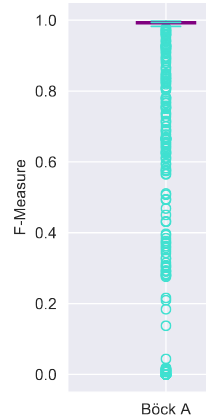
\includegraphics[height=5cm]{./bocka_downbeats.png}
	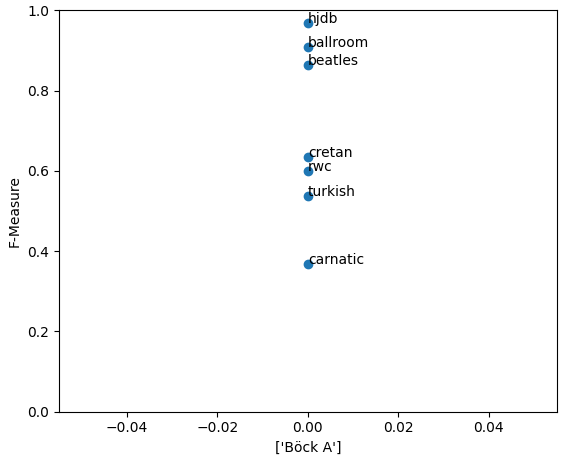
\includegraphics[height=5cm]{./bocka_downbeats_mirex2016.png}
\end{frame}

\note{
	\begin{itemize}
		\item
			Selected 2016 as its the only recent year that had submissions and evaluations for all 3 challenges
		\item
			Adapted the harmonixset plotting code to plot mirex results for BK4
		\item
			My kneejerk reaction was ``HarmonixSet is too easy'', not the case for BK4
		\item
			Labor-intensive to repeat this for each challenge, each algorithm -- only one
	\end{itemize}
}

\begin{frame}[fragile]
	\frametitle{Gangnam style -- HarmonixSet annotations}
	\begin{enumerate}
		\item
		\begin{verbatim}
		# dataset/beats_and_downbeats/0388_gangnamstyle.txt
		0.079   1       1
		0.54    2       1
		1.017   3       1
		1.494   4       1
		1.92    1       2
		2.374545        2       2
		2.82909 3       2
		3.283635        4       2
		\end{verbatim}
		\item
		\begin{verbatim}
		# dataset/segments/0388_gangnamstyle.txt
		0.079    intro
		6.010905 chorus
		14.64726 verse
		\end{verbatim}
		\item
		\href{https://github.com/urinieto/harmonixset/blob/master/dataset/jams/0388_gangnamstyle.jams}{https://github.com/urinieto/harmonixset/blob/master/dataset/jams/0388\_gangnamstyle.jams}\footfullcite{jams}
	\end{enumerate}

\end{frame}

\begin{frame}[fragile]
	\frametitle{Gangnam style results -- beats}
	Beat time output\footfullcite{madmombeats}
	\begin{verbatim}
	beat times: [ 0.09  0.55  1. 1.46 1.91 2.37 2.82 3.28 ... ]
	\end{verbatim}
	vs. HarmonixSet ground truth
	\begin{verbatim}
	0.079   1       1
	0.54    2       1
	1.017   3       1
	1.494   4       1
	1.92    1       2
	2.374545        2       2
	2.82909 3       2
	3.283635        4       2
	\end{verbatim}
	Clicks: \href{run:./gangnam_beats.wav}{BEAT CLICKS}
\end{frame}

\begin{frame}[fragile]
	\frametitle{Gangnam style results -- downbeats}
	Downbeat time output\footfullcite{madmomdownbeats}
	\begin{verbatim}
	downbeat times: [1.0, 2.82, 4.64, 6.46, ...]
	\end{verbatim}
	vs. HarmonixSet ground truth
	\begin{verbatim}
	# awk '{ if ($2 == 3) { print }}' \
	#     dataset/beats_and_downbeats/0388_gangnamstyle.txt
	1.017   3       1
	2.82909 3       2
	4.64727 3       3
	6.46545 3       4
	...
	\end{verbatim}
	Clicks: \href{run:./gangnam_downbeats.wav}{DOWNBEAT CLICKS}
\end{frame}

\note{
	\begin{itemize}
		\item
		 \textbf{NB!} not first beat of bar, but consistently lands on third
	\end{itemize}
}

\begin{frame}[fragile]
	\frametitle{Gangnam style results -- segmentation}
	Structural segmentation output\footfullcite{librosaseg}
	\begin{verbatim}
	segments: [  0.58049887   8.08054422  11.74929705 
            14.09451247 ...
	\end{verbatim}
	vs. HarmonixSet ground truth
	\begin{verbatim}
	0.079 intro 6.010905 chorus 14.64726 verse ...
	\end{verbatim}
	\href{run:./gangnam_segments.wav}{SEGMENT PAUSES}\\
	\href{run:./gangnam_segments_truth.wav}{GROUND TRUTH SEGMENT PAUSES}
\end{frame}

\note{
	\begin{itemize}
		\item
			First 20 second output of the whole processed song
		\item
			Essential that whole song is used as an input. having half the song changes the nature of segmentation. self-similarity, need whole song to know full knowledge
	\end{itemize}
}

\begin{frame}
	\frametitle{Audio alignment}
	YouTube music videos, or different file formats or recordings obtained by researchers, may have temporal differences with the original mp3 files. Alignment data is included to
	\begin{quote}
	... help align the audio in case researchers obtain audio data with different compression formats that might include certain small temporal offsets.
	\end{quote}
	Algorithms used for alignment:
	\begin{enumerate}
		\item
			Dynamic time warping \footfullcite{dtw}, \footfullcite{dtwnotebook}
		\item
			Onsets \footfullcite{librosaonset}
	\end{enumerate}
\end{frame}

\note{
\begin{itemize}
	\item
		DTW in a nutshell:
		\begin{quote}
		DTW has been successfully applied to automatically cope with time deformations and different speeds associated with time-dependent data.
		\end{quote}
	\item
		Onsets don't quite solve the problem, unlike DTW. They're just timestamped information. One would have to do some manual work to compare their onsets to the harmonixset onsets and compute the temporal difference -- or perhaps it can be used as an indicator to run DTW
\end{itemize}
}


\begin{frame}
	\frametitle{Dataset recreation and copyright}
	Data provided to allow independent recreation of dataset includes:\\
	Identifiers in shared music databases:
	\begin{enumerate}
		\item
			MusicBrainz ID \footfullcite{musicbrainz}, open music encyclopedia including unique identifiers for recordings, releases, artists, etc.
		\item
			AcoustID (\href{https://acoustid.org/}{https://acoustid.org/}), open source fingerprinting service to easily match audio content associated with MusicBrainz ids
		\item
			YouTube URLs, including alignment information with the original mp3 files used in the paper
	\end{enumerate}
	Audio/DSP features:
	\begin{enumerate}
		\item
			mel spectrograms for the original mp3 files
		\item
			estimated onsets for the first 30 seconds of audio from librosa
	\end{enumerate}
\end{frame}

\note{
\begin{itemize}
	\item
		Original mp3 files cannot legally be distributed due to copyright
	\item
		Note that these audio features are automated (onsets and spectrograms). This allows independent recreation (aligning the direct output of librosa's onset function on my files and comparing it to their's)
	\item
		Keep in mind onsets are (most likely) essential in beat/downbeat/segmentation tracking. note onsets mark musical events, its a fact. but the raw librosa onset data isn't the opinionated ``algorithm being evaluated'', in this sense its used as a straight feature
\end{itemize}
}

\begin{frame}
	\frametitle{Conclusion}
	\vspace{1em}
	Future work: meta-study to analyze
	\begin{enumerate}
		\item
			Results for algorithms across MIREX challenge datasets
		\item
			Same algorithms applied to the HarmonixSet
		\item
			Comparison of results to gauge the characteristics of the HarmonixSet over established datasets, e.g. in the vein of \cite{mazurkahard}
	\end{enumerate}
	\vspace{1em}
	Source latex and Python code for this presentation: \href{https://gitlab.com/sevagh/MIR-presentations/-/tree/master/01-harmonix-set}{https://gitlab.com/sevagh/MIR-presentations/-/tree/master/01-harmonix-set}
\end{frame}

\note{
	\begin{itemize}
		\item
			HarmonixSet is a high-quality dataset of ground truth annotations for beats, downbeats, and segments in over 900 popular music tracks
		\item
			Stable results from a single set of annotators and techniques (unlike mixing/matching different datasets)
		\item
			Open source, clear repository structure, Jupyter notebooks, approachable and reproducible
	\end{itemize}
}

\end{document}
